% !TeX root = ../main.tex
\section{Topics, Problem Framings, and Platforms}
\subsection{Changing Topics and Persistent Subjects}
Figure~\ref{fig:keytrends} presents selected annual series for RQ1 and RQ2; Appendix~\ref{app:topics} gives the complete distributions. Across the first and last five-edition periods, the networks/diffusion/recommendation component decreases from 16.6\% to 7.8\% of mean topic weight. Search, question answering, and tagging decrease from 11.0\% to 3.2\%, and sentiment/opinion mining from 10.5\% to 4.1\%. Politics/polarization increases from 3.8\% to 11.8\%, and health/social support from 2.8\% to 6.3\%. These are changes in relative composition; a falling share can coexist with continued publication on a subject.

\begin{figure*}[t]
\centering
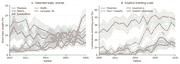
\includegraphics[width=\textwidth]{figures/06_key_trends.png}
\caption{Selected annual topics (A) and problem-framing cues (B). Topic shares describe mean NMF mixture weights; framing-cue rates describe overlapping textual matches. Bands are 95\% within-edition resampling intervals. They reflect composition sensitivity under fixed measures; they do not assess semantic validity.}
\label{fig:keytrends}
\end{figure*}

The language-modeling component reaches 20.5\% in 2026. Small early-period weights reflect shared language and text terms and are not evidence of early generative-AI research. A narrower lexical measure finds explicit LLM/generative-AI terms in 23/161 contributions in 2024 (14.3\%), 41/170 in 2025 (24.1\%), and 61/186 in 2026 (32.8\%). These counts measure visibility in the proceedings, not the prevalence of AI-generated content on social media.

\subsection{Different Problems within Community Research}
The community component's mean share changes little: 10.5\% [8.9, 12.2] in 2007--2011 and 10.0\% [8.8, 11.2] in 2022--2026, an endpoint difference of $-0.5$ percentage points [$-2.6$, 1.5]. Brackets throughout this section denote 95\% resampling intervals.

Governance cues within community-topic weight increase from 4.0\% [0.2, 8.8] to 34.3\% [27.0, 41.4], a difference of 30.3 points [21.8, 38.4]. Figure~\ref{fig:community} shows the annual series. It is uneven, but the endpoint contrast is large.

\begin{figure*}[t]
\centering
\includegraphics[width=\textwidth]{figures/07_community_governance.png}
\caption{Community research and governance framing. Panel A compares the community topic's share of all topic weight with the fraction of community-topic weight attached to papers containing governance cues; these series have different denominators. Panel B repeats the conditional rate after removing governance-matching features before projection onto the fixed topic basis. Bands describe composition sensitivity under the corresponding fixed representation.}
\label{fig:community}
\end{figure*}

Direct vocabulary overlap leaves the contrast largely intact. \emph{Moderation} is one of the community component's twenty leading terms and also matches the governance lexicon. Removing all seven governance-matching features changes the endpoint comparison to 3.6\% [0.1, 8.2] versus 32.5\% [25.3, 39.6], a difference of 28.9 points [20.6, 36.8]. Correlated vocabulary still links the two text-derived measures.

The same pattern survives stricter text checks. Restricting governance cues to the title and first 100 abstract words gives 2.5\% [0.0, 6.6] versus 25.8\% [18.7, 32.6], a difference of 23.2 points [15.1, 31.1]. Excluding papers whose only governance cues are \textit{moderate}, \textit{moderated}, \textit{moderates}, or \textit{moderating}, which often mark statistical or adjectival uses, gives 2.5\% [0.0, 6.6] versus 33.3\% [26.0, 40.4]. Refitting topics on titles and the first 100 abstract words leaves community share at 10.3\% and 9.7\% in the endpoint periods.

\subsection{Harm Framing and Measurement Sensitivity}
Across all contributions, harm/information-integrity cues increase from 6.2\% [3.9, 8.5] to 38.1\% [34.8, 41.2]. Governance cues increase from 1.3\% to 14.8\%, support/well-being cues from 1.3\% to 16.8\%, and prediction/classification cues from 36.3\% to 49.1\%. Table~\ref{tab:periods} uses the same four periods for all selected series.

\begin{table*}[t]
\small
\centering
\begin{tabular}{@{}lrrrr@{}}
\textbf{Measure} & \textbf{2007--2011} & \textbf{2012--2016} & \textbf{2017--2021} & \textbf{2022--2026} \\
\toprule
\rowcolmedium Contributions ($N$) & 386 & 503 & 488 & 762 \\
\hdashline
Networks / diffusion & 16.6 & 13.2 & 10.1 & 7.8 \\
Politics / polarization & 3.8 & 4.8 & 8.7 & 11.8 \\
Communities / participation & 10.5 & 9.2 & 10.0 & 10.0 \\
Health / social support & 2.8 & 4.4 & 6.2 & 6.3 \\
Prediction / classification cues & 36.3 & 42.9 & 47.7 & 49.1 \\
Measurement / validity cues & 8.5 & 15.1 & 15.0 & 18.1 \\
Explanation / intervention cues & 2.1 & 1.4 & 7.6 & 10.5 \\
Harm / integrity cues & 6.2 & 12.3 & 27.0 & 38.1 \\
Governance cues & 1.3 & 1.2 & 6.6 & 14.8 \\
Support / well-being cues & 1.3 & 5.8 & 9.8 & 16.8 \\
Governance within community-topic weight & 4.0 & 1.2 & 14.4 & 34.3 \\
\bottomrule
\end{tabular}
\caption{Selected measures across the same four five-edition periods. All values except $N$ are percentages. The first four rows of measures are mean topic weights; the next six are overlapping cue prevalences. The last row is conditional on community-topic weight. Headline resampling intervals are reported in the text.}
\label{tab:periods}
\end{table*}


\textbf{Abstract length.} Median abstract length increases from 113 words in 2007 to 190 in 2026. With titles plus the first 100 abstract words, harm-cue prevalence changes from 5.7\% [3.4, 8.0] to 31.9\% [28.7, 35.0]. With only the first 100 abstract words, it changes from 5.7\% [3.4, 8.0] to 31.0\% [27.8, 34.1]. The latter difference is 25.3 points [21.5, 29.2], smaller than the full-text difference. Mean harm-cue density also increases, from 0.10 to 0.78 matches per 100 title/abstract words.

\textbf{Historical vocabulary.} Adding trolling, flaming, and vandalism terms leaves the early-period harm estimate at 6.2\% and changes the last-period estimate to 38.3\%. Historical coverage remains uneven: 42.5\% of early contributions match none of the eight categories, compared with 14.0\% in the last period. Period-specific coding is needed to separate changing terminology from changes in framing. Appendix~\ref{app:sensitivity} reports the alternative measures for every period.

\subsection{Platform Context}
Figure~\ref{fig:platforms} addresses the platform dimension of RQ1. Blog mentions decrease from 35.2\% in 2007--2011 to 0.9\% in 2022--2026. Twitter-associated mentions reach a period peak of 45.7\% in 2012--2016 and decline to 24.8\% in 2022--2026. Reddit increases from 1.2\% in 2012--2016 to 15.4\% in 2022--2026. In 2026, Twitter/X and Reddit appear in 15.6\% and 16.1\% of contributions, respectively. These counts describe changing publication contexts; they do not measure platform replacement or equivalent data access.

\begin{figure*}[t]
\centering
\includegraphics[width=\textwidth]{figures/08_platform_shares.png}
\caption{Platform mentions in titles and abstracts for selected long-running contexts, with 95\% composition-resampling bands. Counts can overlap across platforms. The full dictionary contains twenty named families plus weblog terms (Appendix~\ref{app:platforms}).}
\label{fig:platforms}
\end{figure*}

Decentralized platforms have a small, uneven presence in this corpus. Mastodon is mentioned in 0, 3, 0, and 3 papers across 2023--2026; Bluesky in 0, 0, 2, and 3. Publication timing and title/abstract matching limit what these small counts can show.

Annual profiles do not support sharp phase boundaries: no boundary in the baseline five-segment model appears in more than 65\% of 200 resamples. We retain fixed comparison periods; Appendix~\ref{app:boundaries} reports the segmentation diagnostics.
